%% \documentclass[12pt]{article}
%% \usepackage{epsf,amsmath,amssymb,graphicx,axodraw,longtable}
%% \usepackage{lhchiggs,heppennames2,cernunits}
%% \begin{document}

\section{$\PW\PH$/$\PZ\PH$ production mode\footnote{%
    S.~Dittmaier, R.V.~Harlander, J.~Olsen, G.~Piacquadio (eds.);
    O.~Brein, M.~Kr\"amer and T.~Zirke.}}

\subsection{Experimental overview}

Searches for the Higgs boson in the $\PW\PH$ and $\PZ\PH$ production modes,
usually defined as Higgs-strahlung processes, have been considered
mainly by exploiting two decay modes, $\PH \rightarrow \PW^{+}\PW^{-}$ and $\PH
\rightarrow \PQb\bar{\PQb}$. While the former is looked for mainly because it
could contribute to the measurement of the Higgs-boson coupling to $\PW$
bosons, the latter decay mode might contribute to the discovery of a 
low-mass Higgs boson and later allow to measure the coupling of the Higgs
boson to $\PQb$~quarks. The experimental sensitivity to $\PH \rightarrow \PW^{+}\PW^{-}$ 
is highest for Higgs-boson masses above about $160$\UGeV, while the 
$\PH \rightarrow \PQb\bar{\PQb}$ decay modes are investigated for 
the low Higgs-boson mass region, below about $130$\UGeV.

The $\PW\PH \rightarrow \PW\PW\PW$ channel in the tri-lepton mode was explored
with a parton-level study in \Bref{Baer:1998cm}, while a first
estimate of the discovery sensitivity at the LHC was presented in
\Brefs{atlasphystdr,ATL-PHYS-2000-008}, based on
a fast simulation of the ATLAS detector only. In the latter document the
statistical discovery significance of the ATLAS detector with an
integrated luminosity of $30$\Ufb$^{-1}$ was estimated to be above
$3\sigma$ for Higgs-boson masses in the range $160{-}170$\UGeV. However, a
more realistic study based on samples of fully simulated Monte Carlo
events, presented in \Bref{CSC}, shows that the extraction of this
signal might be significantly harder than previously thought, in
particular due to the very high $\PQt\bar{\PQt}$ background, although a
precise quantitative estimate of the discovery significance suffers from
the limited available statistics of the samples and from the fact that
the continuum $\PW\PW\PW$ background was not considered in the study.

The decay channel $\PH \rightarrow \PQb\bar{\PQb}$ is dominant at low
Higgs-boson masses, below about $130$\UGeV. Given the large $\PQb\bar{\PQb}$ 
backgrounds from pure QCD-driven processes, this decay mode is not accessible 
in gluon-fusion production mode and is only marginally accessible 
in combination with the vector-boson fusion. The most promising 
sensitivity studies rely on the associated production of a Higgs boson either with a
$\PZ$ or $\PW$ boson ($\PW\PH$ or $\PZ\PH$) or with a $\PQt\bar{\PQt}$
pair. The $\PW\PH$ and $\PZ\PH$ channels with $\PH \to \PQb\bar{\PQb}$
are the main search channels at the Tevatron for a Higgs boson with low
mass, but at the LHC it is significantly more challenging to extract
these signals from the backgrounds. A first study of the sensitivity to
a Higgs boson in the $\PW\PH$ and $\PZ\PH$ channels was presented in the
ATLAS TDR~\cite{atlasphystdr} and one year later in
\Brefs{ATL-PHYS-2000-023,ATL-PHYS-2000-024}. The channel with the
most significant predicted signal is $\PW\PH$, which however results in
a predicted discovery significance of about $2$ after30\Ufb$^{-1}$ and a signal to background ratio of about $2$\%. Under these conditions, the extraction of the signal is extremely
challenging, since the significance is low and the normalization of the
backgrounds in the signal region must be controlled at the percent level.

More recently, in \Bref{Butterworth:2008iy}, it has been proposed
to focus the search for a Higgs boson in the $\PW\PH$ and $\PZ\PH$
channels with the decay $\PH \rightarrow \PQb\bar{\PQb}$ into the very
specific kinematic region where both the Higgs boson and the $\PW$ or
$\PZ$ boson produced in association with it are emitted at high $\pT$
(e.g.\ $\pT>200$\UGeV), i.e.\ in a topological configuration where they
are back-to-back in the transverse plane and highly boosted. As a first
consequence, the intermediate virtual $\PW$ or $\PZ$ boson producing the
Higgs boson and the associated vector boson must be very massive, thus
even with the LHC center-of-mass energy it will produced quite
centrally, so that the kinematic acceptance of its decay products, the
Higgs and the $\PW$ bosons, will be significantly improved. In addition,
for various reasons, the signal-to-background ratio is significantly
improved, reducing the impact of background uncertainties onto the
discovery significance. A first study based on a realistic simulation of
the ATLAS detector, but based only on $LO$ Monte Carlo generators, was
performed in \Bref{ATL-PHYS-PUB-2009-088}, where it was found that
after 30\Ufb$^{-1}$ of data collected at a center-of-mass energy of
$14\UTeV$ a discovery significance above $3$ should be achievable and that
these channels might contribute, in combination with others, to the
discovery of a low-mass Higgs boson with around 10\Ufb$^{-1}$ of
integrated luminosity.

In the past months the expected sensitivity in the $\PW\PH$ and $\PZ\PH$
channels has been re-evaluated for lower center-of-mass 
energies, by both the ATLAS and CMS Collaborations. With $1\Ufb^{-1}$ of data and 
$\sqrt{s}=7$\UTeV\ ATLAS expects to exclude a Higgs boson at $95\%$ CL 
with a cross section equivalent to about $6$ times the 
SM one~\cite{ATL-PHYS-PUB-2010-015}, 
while with $5\Ufb^{-1}$ of data and $\sqrt{s}=8$\UTeV\ CMS expects to exclude a 
Higgs boson at $95\%$ CL with a cross section equivalent to about
$2$ times the SM one~\cite{CMSPublicPhysicsResultsHIGStandardModelProjectionsWebPage}. 
These results are very preliminary and partially rely on analyses which have not been 
re-optimized for the lower center-of-mass energy.

One of the main challenges of these searches is to control the backgrounds down to
a precision of about $10\%$ or better in the very specific kinematic
region where the signal is expected. Precise differential predictions 
for these backgrounds as provided by theoretical perturbative calculations and parton-shower 
Monte Carlo generators are therefore crucial. Further studies (e.g.\ in
\Bref{CERN-THESIS-2010-027}) suggest that with data corresponding to 
an integrated luminosity of the order of 30\Ufb$^{-1}$ the $\PQt\bar{\PQt}$
background might be extracted from data in a signal-free control region, 
while this seems to be significantly harder for the $\PW\PQb\bar{\PQb}$ or
$\PZ\PQb\bar{\PQb}$ irreducible backgrounds, even in the presence of such a 
large amount of data.

For all search channels previously mentioned, a precise prediction of the
signal cross section and of the kinematic properties of the produced
final-state particles is of utmost importance, together with a possibly
accurate estimation of the connected systematic uncertainties.  The
scope of this section is to present the state-of-the-art inclusive cross
sections for the $\PW\PH$ and $\PZ\PH$ Higgs-boson production modes at different
LHC center-of-mass energies and for different possible values of the
Higgs-boson mass and their connected uncertainties.
%in case we will have this...
%Some first preliminary results 
%of differential properties of the Higgs boson in these production modes and their connected uncertainties 
%will be presented as well.

\subsection{Theoretical framework}

The inclusive partonic cross section for associated production of a
Higgs boson ($\PH$) and a weak gauge boson ($V$) can be written as
\begin{equation}
\begin{split}
\hat \sigma(\hat s) = \int_0^{\hat s} {\rm d}k^2 \,
\sigma(V^\ast(k))\,\frac{{\rm d}\Gamma}{{\rm d}k^2} (V^\ast(k)\to \PH V) +
\Delta\sigma\,,
\label{eq:sigpart}
\end{split}
\end{equation}
where $\sqrt{\hat s}$ is the partonic center-of-mass energy.
The first term on the r.h.s.\ arises from terms where a virtual gauge
boson $V^\ast$ with momentum $k$ is produced in a Drell--Yan-like
process, which then radiates a Higgs boson. The factor $\sigma(V^\ast)$
is the total cross section for producing the intermediate vector boson
and is fully analogous to the Drell--Yan expression. The second term on
the r.h.s., $\Delta\sigma$, comprises all remaining contributions.
The hadronic cross section is obtained from the partonic expression of
Eq.\,(\ref{eq:sigpart}) by convoluting it with the parton densities in
the usual way.

The LO prediction for $pp\to V\PH$ ($V=\PW,\PZ$) is based on the Feynman
diagrams shown in \Fref{fig:ppVH-LO-diags}\,(a),(b) and leads to a
LO cross section of ${\cal O}(\GF^2)$.
\begin{figure}
\begin{center}
\begin{tabular}{ccc}
{\unitlength 1pt \SetScale{1}
\begin{picture}(150,100)(-5,-10)
\ArrowLine(20, 5)(50,40)
\ArrowLine(50,40)(20,75)
\Photon(50,40)(90,40){2}{5}
\Photon(120,20)(90,40){2}{5}
\DashLine(90,40)(120,60){5}
\Vertex(50,40){2}
\Vertex(90,40){2}
\put( -4, 2){${\PQu/\PQd}$}
\put( -4,72){$\PAQd/\PAQu$}
\put(125,56){${\PH}$}
\put( 62,25){${\PW}$}
\put(125,12){${\PW^\pm}$}
\end{picture}
}\hspace*{-2em} &
{\unitlength 1pt \SetScale{1}
\begin{picture}(150,100)(-5,-10)
\ArrowLine(20, 5)(50,40)
\ArrowLine(50,40)(20,75)
\Photon(50,40)(90,40){2}{5}
\Photon(120,20)(90,40){2}{5}
\DashLine(90,40)(120,60){5}
\Vertex(50,40){2}
\Vertex(90,40){2}
\put(  8, 2){${\PQq}$}
\put(  8,72){${\PAQq}$}
\put(125,56){${\PH}$}
\put( 65,25){${\PZ}$}
\put(125,12){${\PZ}$}
\end{picture}
}\hspace*{-2em} &
{\unitlength 1pt \SetScale{1}
\begin{picture}(150,100)(-5,-10)
\Gluon(50,15)(20, 5){4}{3}
\Gluon(20,75)(50,65){4}{3}
\ArrowLine(50,65)(50,15)
\ArrowLine(90,65)(50,65)
\ArrowLine(50,15)(90,15)
\ArrowLine(90,15)(90,65)
\Photon(120,10)(90,15){2}{5}
\DashLine(90,65)(120,70){5}
\Vertex(90,65){2}
\Vertex(90,15){2}
\Vertex(50,15){2}
\Vertex(50,65){2}
\put(  55, 35){$\PQt$}
\put(  8, 2){$\Pg$}
\put(  8,72){$\Pg$}
\put(125,68){$\PH$}
\put(125,7){$\PZ$}
\end{picture}
}\\
(a) & (b) & (c)
\end{tabular}
\end{center}
\vspace*{-1em}
\caption{(a), (b) LO diagrams for the partonic processes $\Pp\Pp\to V\PH$
  ($V=\PW,\PZ$); (c) diagram contributing to the $\Pg\Pg\to \PH\PZ$ channel.}
\label{fig:ppVH-LO-diags}
\end{figure}
Through NLO, the QCD
corrections are fully given by the NLO QCD corrections to the Drell--Yan
cross section $\hat
\sigma(V^\ast)$~\cite{Han:1991ia,Baer:1992vx,Ohnemus:1992bd}. For $V=\PW$,
this observation carries over to NNLO%
\footnote{\samepage This statement holds up to two-loop diagrams where the Higgs
  boson is attached to a one-loop Drell--Yan diagram via the loop-induced
  $\Pg\Pg\PH$ coupling. Such diagrams, which are neglected so far, are believed 
  to have only a small impact; their calculation is in progress.},
so that the corresponding QCD
corrections can be easily derived by integrating the classic Drell--Yan
result~\cite{Hamberg:1990np,Harlander:2002wh} over the virtuality of the
intermediate gauge boson. For that purpose, the program {\sc VH@NNLO}
has been developed~\cite{Brein:2003wg}, building on the publicly
available code {\sc zwprod.f}~\cite{Hamberg:1990np}.

The Drell--Yan-like corrections that determine the NNLO result for
$\PW\PH$ production also give the bulk of the $\PZ\PH$
contribution. However, in that case, there are gluon--gluon-induced
terms that do not involve a virtual weak gauge boson; both $\PZ$ and
$\PH$ couple to the gluons via a top-quark loop in this case, see
\Fref{fig:ppVH-LO-diags}\,(c). This class of diagrams is not taken
into account in {\sc VH@NNLO}; it was computed in
\Bref{Brein:2003wg}, and the numbers included in the results below are based on
the corresponding numerical code.

As every hadron collider observable that is evaluated at fixed order
perturbation theory, the cross section depends on the unphysical
renormalization and factorization scales $\mu_R$ and $\mu_F$.  Since the
QCD corrections mostly affect the production of the intermediate gauge
boson, a natural choice for the central value of $\mu_F$ and $\mu_R$ is
the virtuality $k^2$ of this gauge boson.

NLO electroweak (EW) corrections have been evaluated in
\Bref{Ciccolini:2003jy}.  In contrast to the NLO QCD corrections,
EW corrections do not respect a factorization into
Drell--Yan-like production and decay, since there are irreducible (box)
corrections to $\PQq\PQq^{(\prime)}\to V\PH$ already at one loop.  Note also
that the size of the EW corrections (as usual) sensitively
depend on the chosen renormalization scheme to define the weak
couplings, most notably on the choice for the electromagnetic couplings
$\alpha$. The preferred choice, which should be most robust with
respect to higher-order corrections, is the so-called $\GF$ scheme,
where $\alpha$ is derived from Fermi's constant $\GF$.

The combination of QCD and EW corrections poses
the question on whether factorization of the
EW and QCD effects is a valid approximation to the actual
mixed ${\cal O}(\GF\alphas)$ corrections. Following \Bref{Brein:2004ue},
we present our result based
on the assumption that full factorization of the two effects is valid,
i.e., the cross section is determined as
\begin{equation}
\begin{split}
\sigma_{\PW\PH} = \sigma_{\PW\PH}^{\mbox{\footnotesize\sc VH@NNLO}} 
\times (1 + \delta_{\PW\PH,\rm EW})\,, \qquad
\sigma_{\PZ\PH} = \sigma_{\PZ\PH}^{\mbox{\footnotesize\sc VH@NNLO}} 
\times (1 + \delta_{\PZ\PH,\rm EW})
+\sigma_{\Pg\Pg\to\PZ\PH} \,,
\end{split}
\end{equation}
where $\sigma_{V\PH}^{\mbox{\footnotesize\sc VH@NNLO}}$ 
is the NNLO QCD result of {\sc VH@NNLO} 
through ${\cal O}(\alphas^2)$, $\delta_{V\PH,\rm EW}$ is the relative 
EW correction factor determined in the limit $\alphas=0$, and
$\sigma_{\Pg\Pg\to\PZ\PH}$ is the NNLO contribution 
to $\PZ\PH$ production induced by $\Pg\Pg$ fusion.

The PDF+$\alphas$ uncertainties are evaluated according to the recipe
proposed in Section~\ref{sec:pdf4lhcreco} of this report. The
uncertainties due to the residual dependence on the renormalization and
factorization scales are determined by considering the cross section
when mutually fixing one of $\mu_R$ and $\mu_F$ at the central scale
$\sqrt{k^2}$ (the mass of the intermediate gauge boson, see above), and varying
the other scale between $\sqrt{k^2}/3$ and $3\sqrt{k^2}$.
The EW factor $\delta_{V\PH,\rm EW}$ is always calculated in the same way as
the central value of the cross section, because the relative EW correction
is insensitive to the PDF and/or scale choices.

In principle there are also real NLO EW corrections induced by
initial-state photons, which are ignored, since current PDF sets do not
deliver a photon PDF.  The photon PDF is, however, strongly suppressed,
so that an uncertainty of not more than 1\% should arise from this
approximation.  This estimated percent uncertainty, which rests on the
comparison with other cross sections such as vector-boson
fusion~\cite{Ciccolini:2007ec,Ciccolini:2007jr} where these effects have
been calculated, also includes the neglect of NLO EW corrections in the
evolution of current PDFs.

\subsection{Numerical results}

The results for the NLO and the NNLO QCD cross sections for $\PW\PH$
production, including NLO EW effects, are shown in
\Fref{fig:wh-xsec}, both at $7\UTeV$ and $14\UTeV$. The numbers are obtained
by summing over $\PWp\PH$ and $\PWm\PH$ production.
The corresponding $K$-factors, obtained by normalizing the cross section
to the LO value (at central scales and PDFs), are shown in
\Fref{fig:wh-k}. The little kinks at around 160\UGeV\ and, somewhat
smaller, 180\UGeV\ are due to the $\PW\PW$ and $\PZ\PZ$ thresholds that occur
in the EW radiative corrections (see also \Bref{Ciccolini:2003jy}).
The present prediction does not properly describe the threshold
behaviour, which is in fact singular on threshold. Therefore, 
in practice, Higgs mass windows of $\sim \pm 5\UGeV$ around the 
thresholds should be obtained upon
interpolation unless the threshold regions are properly described
(e.g.\ by complex masses), a task which is in progress.
The uncertainty of the threshold interpolation is about 1\%.

The plots for $\PZ\PH$ production are shown in \Frefs{fig:zh-xsec}
and \ref{fig:zh-k}. The fact that the uncertainty bands at NNLO are of
the same order of magnitude as at NLO is due to the $\Pg\Pg$ channel
that occurs only at NNLO and is absent in the $\PW\PH$ case.
In more detail, for the centre-of-mass energy of $7\UTeV$ ($14\UTeV$) the
$\Pg\Pg$ channel contributes to $\PZ\PH$ production by
$2{-}6\%$ ($4{-}12\%$) with an uncertainty of 
$20{-}30\%$ from scale variation and of $4\%$ ($2\%$) from PDF, 
translating roughly into a $0.5{-}1.5\%$
($1{-}3\%$) uncertainty on the full result.

We have checked the NLO numbers against {\sc V2HV}~\cite{V2HV} and find
agreement at the permille level, once CKM mixing is included in {\sc
  V2HV}. Also, we find satisfactory agreement of the NLO result when
comparing to {\sc MCFM}~\cite{MCFM}. However, the comparison is less strict in
this case as {\sc MCFM} does not allow the same scale choice as used here.

The results for the central values of the cross section and the
corresponding theoretical uncertainties are shown in
\Trefs{tab:wzh7} and \ref{tab:wzh14} for $7\UTeV$ and $14\UTeV$,
respectively. Notice that the scale uncertainties for $\PZ\PH$ production
are consistently larger than for $\PW\PH$ production, because they are
dominated by the uncertainties of the $\Pg\Pg$ channel.

\begin{figure}
\vspace{0pt}
\begin{center}
\begin{tabular}{cc}
\includegraphics[%bb=20 270 550 820,
angle=0,width=.46\linewidth]{YRHXS_WHZH/YRHXS_WHZH_fig2.eps} &
\includegraphics[%bb=20 270 550 820,
angle=0,width=.46\linewidth]{YRHXS_WHZH/YRHXS_WHZH_fig1.eps}\\[-1.5em] 
(a) & (b)
\end{tabular}
\end{center}
\vspace*{-1em}
\caption[]{\label{fig:wh-xsec} Cross section for the sum of $\PWp\PH$
  and $\PWm\PH$ production for $7\UTeV$ and $14\UTeV$ at (a) NLO and (b) NNLO
  QCD, including NLO EW effects in both cases.}
%\end{figure}
%
%\begin{figure}
\vspace{0pt}
\begin{center}
\begin{tabular}{cc}
\includegraphics[%bb=20 270 550 820,
angle=0,width=.46\linewidth]{YRHXS_WHZH/YRHXS_WHZH_fig4.eps} &
\includegraphics[%bb=20 270 550 820,
angle=0,width=.46\linewidth]{YRHXS_WHZH/YRHXS_WHZH_fig3.eps}\\[-1.5em] 
(a) & (b)\\[.5em]
\includegraphics[%bb=20 270 550 820,
angle=0,width=.46\linewidth]{YRHXS_WHZH/YRHXS_WHZH_fig6.eps} &
\includegraphics[%bb=20 270 550 820,
angle=0,width=.46\linewidth]{YRHXS_WHZH/YRHXS_WHZH_fig5.eps}\\[-1.5em] 
(c) & (d)
\end{tabular}
\end{center}
\vspace*{-1em}
\caption[]{\label{fig:wh-k}$K$-factors (ratio to LO prediction) for the
  NLO and NNLO cross sections of \Fref{fig:wh-xsec}.}
\end{figure}

\begin{figure}
\vspace{0pt}
\begin{center}
\begin{tabular}{cc}
\includegraphics[%bb=20 270 550 820,
angle=0,width=.46\linewidth]{YRHXS_WHZH/YRHXS_WHZH_fig8.eps} &
\includegraphics[%bb=20 270 550 820,
angle=0,width=.46\linewidth]{YRHXS_WHZH/YRHXS_WHZH_fig7.eps}\\[-1.5em]  
(a) & (b)
\end{tabular}
\end{center}
\vspace*{-1em}
\caption[]{\label{fig:zh-xsec} Cross section for $\PZ\PH$
  production for $7\UTeV$ and $14\UTeV$ at (a) NLO and (b) NNLO
  QCD, including NLO EW effects in both cases.}
%\end{figure}
%
%\begin{figure}
\vspace{0pt}
\begin{center}
\begin{tabular}{cc}
\includegraphics[%bb=20 270 550 820,
angle=0,width=.46\linewidth]{YRHXS_WHZH/YRHXS_WHZH_fig10.eps} &
\includegraphics[%bb=20 270 550 820,
angle=0,width=.46\linewidth]{YRHXS_WHZH/YRHXS_WHZH_fig9.eps}\\[-1.5em]  
(a) & (b)\\[.5em]
\includegraphics[%bb=20 270 550 820,
angle=0,width=.46\linewidth]{YRHXS_WHZH/YRHXS_WHZH_fig12.eps} &
\includegraphics[%bb=20 270 550 820,
angle=0,width=.46\linewidth]{YRHXS_WHZH/YRHXS_WHZH_fig11.eps}\\[-1.5em]  
(c) & (d)
\end{tabular}
\end{center}
\vspace*{-1em}
\caption[]{\label{fig:zh-k}$K$-factors (ratio to LO prediction) for the
  NLO and NNLO cross sections of \Fref{fig:zh-xsec}.}
\end{figure}

\begin{table}
%  \vspace{-\headsep}
   \begin{center}
   \caption[]{\label{tab:wzh7}Total inclusive cross section at $7\UTeV$ for
  $\PW\PH$ and $\PZ\PH$ production at NNLO QCD + NLO EW. The first error
  indicates the uncertainty from the renormalization and factorization
  scale variation, the second from the PDF+$\alphas$ variation.}
%    \include{YRHXS_WHZH/wzh7nnlo}
   \small
   \begin{tabular}{ccccccc}
   \hline
$\MH[\UGeVZ]$ & $\sigma(\PW\PH)[\UpbZ]$ & Scale [\%] & PDF4LHC [\%] &
$\sigma(\PZ\PH)[\UpbZ]$ & Scale [\%] & PDF4LHC [\%]
\\ \hline
$ 90 $ & $    1.640 $ & $ +0.3   -\!0.8  $ & 
$ \pm 3.0 $
 & $   0.8597 $ & $ +0.9   -\!1.0  $ &
$ \pm 3.0 $ \\[.2em]

$ 95 $ & $    1.392 $ & $ +0.1   -\!0.9  $ & 
$ \pm 3.2 $
 & $   0.7348 $ & $ +1.0   -\!1.1  $ &
$ \pm 3.6 $ \\[.2em]

$ 100 $ & $    1.186 $ & $ +0.6   -\!0.5  $ & 
$ \pm 3.4 $
 & $   0.6313 $ & $ +1.1   -\!1.2  $ &
$ \pm 3.4 $ \\[.2em]

$ 105 $ & $    1.018 $ & $ +0.3   -\!0.8  $ & 
$ \pm 3.5 $
 & $   0.5449 $ & $ +1.3   -\!1.6  $ &
$ \pm 3.7 $ \\[.2em]

$ 110 $ & $   0.8754 $ & $ +0.3   -\!0.7  $ & 
$ \pm 3.8 $
 & $   0.4721 $ & $ +1.2   -\!1.2  $ &
$ \pm 4.1 $ \\[.2em]

$ 115 $ & $   0.7546 $ & $ +0.4   -\!0.8  $ & 
$ \pm 3.9 $
 & $   0.4107 $ & $ +1.3   -\!1.2  $ &
$ \pm 4.2 $ \\[.2em]

$ 120 $ & $   0.6561 $ & $ +0.4   -\!0.7  $ & 
$ \pm 3.4 $
 & $   0.3598 $ & $ +1.5   -\!1.2  $ &
$ \pm 3.5 $ \\[.2em]

$ 125 $ & $   0.5729 $ & $ +0.2   -\!0.8  $ & 
$ \pm 3.5 $
 & $   0.3158 $ & $ +1.4   -\!1.6  $ &
$ \pm 3.5 $ \\[.2em]

$ 130 $ & $   0.5008 $ & $ +0.3   -\!0.8  $ & 
$ \pm 3.5 $
 & $   0.2778 $ & $ +1.5   -\!1.4  $ &
$ \pm 3.7 $ \\[.2em]

$ 135 $ & $   0.4390 $ & $ +0.7   -\!0.4  $ & 
$ \pm 3.4 $
 & $   0.2453 $ & $ +1.7   -\!1.4  $ &
$ \pm 3.6 $ \\[.2em]

$ 140 $ & $   0.3857 $ & $ +0.5   -\!0.5  $ & 
$ \pm 3.5 $
 & $   0.2172 $ & $ +1.5   -\!1.6  $ &
$ \pm 3.7 $ \\[.2em]

$ 145 $ & $   0.3406 $ & $ +0.2   -\!0.8  $ & 
$ \pm 3.8 $
 & $   0.1930 $ & $ +1.8   -\!1.8  $ &
$ \pm 4.0 $ \\[.2em]

$ 150 $ & $   0.3001 $ & $ +0.4   -\!0.8  $ & 
$ \pm 3.3 $
 & $   0.1713 $ & $ +1.8   -\!1.6  $ &
$ \pm 3.6 $ \\[.2em]

$ 155 $ & $   0.2646 $ & $ +0.5   -\!0.8  $ & 
$ \pm 3.5 $
 & $   0.1525 $ & $ +2.1   -\!1.6  $ &
$ \pm 3.6 $ \\[.2em]

$ 160 $ & $   0.2291 $ & $ +0.5   -\!0.7  $ & 
$ \pm 3.8 $
 & $   0.1334 $ & $ +2.0   -\!1.7  $ &
$ \pm 4.0 $ \\[.2em]

$ 165 $ & $   0.2107 $ & $ +0.5   -\!0.7  $ & 
$ \pm 3.6 $
 & $   0.1233 $ & $ +2.1   -\!1.7  $ &
$ \pm 4.1 $ \\[.2em]

$ 170 $ & $   0.1883 $ & $ +0.5   -\!0.7  $ & 
$ \pm 3.8 $
 & $   0.1106 $ & $ +2.2   -\!1.9  $ &
$ \pm 4.2 $ \\[.2em]

$ 175 $ & $   0.1689 $ & $ +0.3   -\!1.1  $ & 
$ \pm 3.8 $
 & $  0.09950 $ & $ +2.1   -\!1.9  $ &
$ \pm 4.1 $ \\[.2em]

$ 180 $ & $   0.1521 $ & $ +0.6   -\!0.6  $ & 
$ \pm 3.5 $
 & $  0.08917 $ & $ +2.2   -\!1.9  $ &
$ \pm 3.8 $ \\[.2em]

$ 185 $ & $   0.1387 $ & $ +0.4   -\!0.9  $ & 
$ \pm 3.5 $
 & $  0.08139 $ & $ +2.3   -\!2.0  $ &
$ \pm 3.8 $ \\[.2em]

$ 190 $ & $   0.1253 $ & $ +0.5   -\!0.7  $ & 
$ \pm 3.7 $
 & $  0.07366 $ & $ +2.2   -\!2.1  $ &
$ \pm 3.9 $ \\[.2em]

$ 195 $ & $   0.1138 $ & $ +0.7   -\!0.6  $ & 
$ \pm 3.7 $
 & $  0.06699 $ & $ +2.3   -\!1.9  $ &
$ \pm 4.0 $ \\[.2em]

$ 200 $ & $   0.1032 $ & $ +0.4   -\!1.0  $ & 
$ \pm 3.8 $
 & $  0.06096 $ & $ +2.3   -\!1.9  $ &
$ \pm 4.1 $ \\[.2em]

$ 210 $ & $  0.08557 $ & $ +0.5   -\!0.7  $ & 
$ \pm 3.7 $
 & $  0.05068 $ & $ +2.1   -\!2.0  $ &
$ \pm 4.2 $ \\[.2em]

$ 220 $ & $  0.07142 $ & $ +0.3   -\!0.9  $ & 
$ \pm 3.7 $
 & $  0.04235 $ & $ +2.2   -\!1.9  $ &
$ \pm 4.2 $ \\[.2em]

$ 230 $ & $  0.06006 $ & $ +0.7   -\!0.7  $ & 
$ \pm 4.5 $
 & $  0.03560 $ & $ +2.1   -\!1.9  $ &
$ \pm 4.8 $ \\[.2em]

$ 240 $ & $  0.05075 $ & $ +0.5   -\!0.7  $ & 
$ \pm 4.0 $
 & $  0.02999 $ & $ +1.9   -\!1.8  $ &
$ \pm 4.4 $ \\[.2em]

$ 250 $ & $  0.04308 $ & $ +0.5   -\!0.7  $ & 
$ \pm 4.0 $
 & $  0.02540 $ & $ +2.0   -\!1.6  $ &
$ \pm 4.2 $ \\[.2em]

$ 260 $ & $  0.03674 $ & $ +0.8   -\!0.7  $ & 
$ \pm 4.0 $
 & $  0.02158 $ & $ +1.8   -\!1.7  $ &
$ \pm 4.5 $ \\[.2em]

$ 270 $ & $  0.03146 $ & $ +0.6   -\!0.9  $ & 
$ \pm 3.8 $
 & $  0.01839 $ & $ +1.7   -\!1.7  $ &
$ \pm 4.3 $ \\[.2em]

$ 280 $ & $  0.02700 $ & $ +0.4   -\!1.0  $ & 
$ \pm 4.4 $
 & $  0.01575 $ & $ +1.6   -\!1.3  $ &
$ \pm 4.9 $ \\[.2em]

$ 290 $ & $  0.02333 $ & $ +0.7   -\!0.8  $ & 
$ \pm 4.2 $
 & $  0.01355 $ & $ +1.5   -\!1.3  $ &
$ \pm 4.5 $ \\[.2em]

$ 300 $ & $  0.02018 $ & $ +0.6   -\!0.9  $ & 
$ \pm 4.5 $
 & $  0.01169 $ & $ +1.4   -\!1.2  $ &
$ \pm 5.0 $ \\[.2em]

   \hline
   \end{tabular}
   \end{center}
\end{table}

\begin{table}
%    \vspace{-\headsep}
    \begin{center}
      \caption[]{\label{tab:wzh14}Total inclusive cross section at
  14\UTeV\ for $\PW\PH$ and $\PZ\PH$ production at NNLO QCD + NLO
  EW. The first error indicates the uncertainty from the renormalization
  and factorization scale variation, the second from the PDF+$\alphas$
  variation.}
%      \include{YRHXS_WHZH/wzh14nnlo}
   \small
   \begin{tabular}{ccccccc}
   \hline
$\MH[\UGeVZ]$ & $\sigma(\PW\PH)[\UpbZ]$ & Scale [\%] & PDF4LHC [\%] &
$\sigma(\PZ\PH)[\UpbZ]$ & Scale [\%] & PDF4LHC [\%]
\\ \hline
$ 90 $ & $    4.090 $ & $   +0.4   -\!0.7  $ & 
$ \pm 3.9 $
 & $    2.245 $ & $  +1.3   -\!1.7  $ &
$ \pm 4.0 $ \\[.2em]

$ 95 $ & $    3.499 $ & $   +0.6   -\!0.7  $ & 
$ \pm 3.8 $
 & $    1.941 $ & $   +1.6   -\!1.6  $ &
$ \pm 3.6 $ \\[.2em]

$ 100 $ & $    3.002 $ & $   +0.8   -\!0.6  $ & 
$ \pm 3.7 $
 & $    1.683 $ & $   +1.9   -\!1.5  $ &
$ \pm 3.8 $ \\[.2em]

$ 105 $ & $    2.596 $ & $   +0.6   -\!0.5  $ & 
$ \pm 3.5 $
 & $    1.468 $ & $   +1.7   -\!1.7  $ &
$ \pm 3.7 $ \\[.2em]

$ 110 $ & $    2.246 $ & $   +0.3   -\!0.8  $ & 
$ \pm 3.8 $
 & $    1.283 $ & $   +2.1   -\!1.6  $ &
$ \pm 4.0 $ \\[.2em]

$ 115 $ & $    1.952 $ & $   +0.7   -\!0.2  $ & 
$ \pm 3.8 $
 & $    1.130 $ & $   +2.5   -\!1.5  $ &
$ \pm 3.7 $ \\[.2em]

$ 120 $ & $    1.710 $ & $   +0.6   -\!0.3  $ & 
$ \pm 3.8 $
 & $   0.9967 $ & $   +2.4   -\!1.8  $ &
$ \pm 3.6 $ \\[.2em]

$ 125 $ & $    1.504 $ & $   +0.3   -\!0.6  $ & 
$ \pm 3.8 $
 & $   0.8830 $ & $   +2.7   -\!1.8  $ &
$ \pm 3.7 $ \\[.2em]

$ 130 $ & $    1.324 $ & $   +0.5   -\!0.4  $ & 
$ \pm 3.3 $
 & $   0.7846 $ & $   +2.9   -\!1.8  $ &
$ \pm 3.4 $ \\[.2em]

$ 135 $ & $    1.167 $ & $   +0.6   -\!0.5  $ & 
$ \pm 2.9 $
 & $   0.6981 $ & $   +2.9   -\!2.2  $ &
$ \pm 3.0 $ \\[.2em]

$ 140 $ & $    1.034 $ & $   +0.2   -\!0.7  $ & 
$ \pm 3.1 $
 & $   0.6256 $ & $   +2.8   -\!2.2  $ &
$ \pm 3.0 $ \\[.2em]

$ 145 $ & $   0.9200 $ & $   +0.5   -\!0.4  $ & 
$ \pm 3.3 $
 & $   0.5601 $ & $   +3.3   -\!2.1  $ &
$ \pm 3.4 $ \\[.2em]

$ 150 $ & $   0.8156 $ &  $  +0.3   -\!0.6  $ & 
$ \pm 2.7 $
 & $   0.5016 $ & $   +3.3   -\!2.0  $ &
$ \pm 2.7 $ \\[.2em]

$ 155 $ & $   0.7255 $ &  $  +0.4   -\!0.6  $ & 
$ \pm 3.1 $
 & $   0.4513 $ & $   +3.3   -\!2.4  $ &
$ \pm 3.2 $ \\[.2em]

$ 160 $ & $   0.6341 $ &  $  +0.2   -\!0.5  $ & 
$ \pm 3.1 $
 & $   0.3986 $ & $   +3.5   -\!2.4  $ &
$ \pm 3.1 $ \\[.2em]

$ 165 $ & $   0.5850 $ &  $  +0.2   -\!0.6  $ & 
$ \pm 2.4 $
 & $   0.3705 $ & $   +3.8   -\!2.3  $ &
$ \pm 2.6 $ \\[.2em]

$ 170 $ & $   0.5260 $ &  $  +0.3   -\!0.7  $ & 
$ \pm 2.8 $
 & $   0.3355 $ & $   +3.5   -\!2.4  $ &
$ \pm 3.0 $ \\[.2em]

$ 175 $ & $   0.4763 $ &  $  +0.5   -\!0.3  $ & 
$ \pm 2.9 $
 & $   0.3044 $ & $   +3.5   -\!2.6  $ &
$ \pm 3.1 $ \\[.2em]

$ 180 $ & $   0.4274 $ & $   +0.4   -\!0.6  $ & 
$ \pm 2.8 $
 & $   0.2744 $ & $   +3.7   -\!2.8  $ &
$ \pm 3.0 $ \\[.2em]

$ 185 $ & $   0.3963 $ & $   +0.4   -\!0.7  $ & 
$ \pm 2.5 $
 & $   0.2524 $ & $   +3.5   -\!2.9  $ &
$ \pm 2.6 $ \\[.2em]

$ 190 $ & $   0.3600 $ & $   +0.2   -\!0.6  $ & 
$ \pm 2.8 $
 & $   0.2301 $ & $  +3.5   -\!2.9  $ &
$ \pm 3.0 $ \\[.2em]

$ 195 $ & $   0.3291 $ & $   +0.3   -\!0.7  $ & 
$ \pm 2.7 $
 & $   0.2112 $ & $  +3.5   -\!2.9  $ &
$ \pm 2.9 $ \\[.2em]

$ 200 $ & $   0.3004 $ & $   +0.4   -\!0.5  $ & 
$ \pm 3.0 $
 & $   0.1936 $ & $  +3.6   -\!3.0  $ &
$ \pm 3.1 $ \\[.2em]

$ 210 $ & $   0.2526 $ & $   +0.2   -\!0.7  $ & 
$ \pm 2.6 $
 & $   0.1628 $ & $  +3.9   -\!2.5  $ &
$ \pm 2.6 $ \\[.2em]

$ 220 $ & $   0.2138 $ & $   +0.6   -\!0.5  $ & 
$ \pm 2.8 $
 & $   0.1380 $ & $   +3.4   -\!2.7  $ &
$ \pm 2.9 $ \\[.2em]

$ 230 $ & $   0.1826 $ & $   +0.4   -\!0.5  $ & 
$ \pm 3.5 $
 & $   0.1173 $ & $   +3.4   -\!2.6  $ &
$ \pm 3.6 $ \\[.2em]

$ 240 $ & $   0.1561 $ & $   +0.4   -\!0.5  $ & 
$ \pm 3.3 $
 & $  0.09996 $ & $   +3.1   -\!2.5  $ &
$ \pm 3.4 $ \\[.2em]

$ 250 $ & $   0.1343 $ & $   +0.2   -\!0.7  $ & 
$ \pm 3.0 $
 & $  0.08540 $ & $  +3.0   -\!2.3  $ &
$ \pm 3.2 $ \\[.2em]

$ 260 $ & $   0.1161 $ & $   +0.2   -\!0.7  $ & 
$ \pm 2.8 $
 & $  0.07341 $ & $  +3.0   -\!2.1  $ &
$ \pm 3.1 $ \\[.2em]

$ 270 $ & $   0.1009 $ & $   +0.5   -\!0.6  $ & 
$ \pm 2.6 $
 & $  0.06325 $ & $  +2.5   -\!1.9  $ &
$ \pm 2.8 $ \\[.2em]

$ 280 $ & $  0.08781 $ & $   +0.4   -\!0.6  $ & 
$ \pm 3.0 $
 & $  0.05474 $ & $  +2.5   -\!1.8  $ &
$ \pm 3.2 $ \\[.2em]

$ 290 $ & $  0.07714 $ & $   +0.3   -\!0.6  $ & 
$ \pm 3.2 $
 & $  0.04769 $ & $  +2.2   -\!1.5  $ &
$ \pm 3.2 $ \\[.2em]

$ 300 $ & $  0.06755 $ & $   +0.6   -\!0.5  $ & 
$ \pm 3.3 $
 & $  0.04156 $ & $   +2.0   -\!1.6  $ &
$ \pm 3.6 $ \\[.2em]

   \hline
   \end{tabular}
   \end{center}
\end{table}

\clearpage


%% \bibliographystyle{atlasnote}
%% \bibliography{YRHXS_bib}

%% \end{document}
